\section{ElSe im Test}
Der Ursprüngliche ElSe-Algorithmus wurde für Eye-Tracking Brillen entwickelt, also für ein qualitativ hochwertiges Bild eines Auges, daher soll geprüft werden in wieweit es in dieser Anwendung eingesetzt werden kann.\\
Um die einzelnen Grau-Verfahren besser vergleichen zu können, wurden künstliche Augen aus dem Datensatz \cite{database_Eye} verwendet damit die exakte Position der Landmarks bekannt ist.\\
Ein gutes Verfahren muss stabil gegenüber der Skalierung sein, damit es auch auf kleinen Bereichen zuverlässig arbeitet. Da für die spätere Anwendung vor allem das Zentrum der Pupille von Interesse ist, wird der euklidische Abstand zum Zentrum als Qualitätsmaß verwendet.\\
Da ElSe für Eye-Tracking Brillen entwickelt wurde ist der Augenbereich genauer bestimmt als im Datensatz enthalten, daher wurde der Bildbereich soweit verkleinert, dass nur noch alle Landmarks des Auges mit etwas Rand dargestellt werden, um diesen Anforderungen entsprechend nahe zu kommen.\\
Somit sind die Bildausschnitte im Datensatz auf denen gerechnet wird etwa 64 auf 29 Pixel groß und werden für die Verarbeitung auf eine Breite von 384 Pixeln vergrößert, die Auflösung, wofür ElSe entwickelt wurde. Da durch die Skalierung allerdings keine zusätzlichen Informationen entstehen, ist vor allem die grobe Bestimmung der Ellipse, beschrieben in \autoref{ElSe_Grob}, von Interesse. Diese Auswahl des Bildbereiches kann auch in der späteren Anwendung eingesetzt werden, da der Augenbereich durch eigene Landmarks in der Gesichtsanalyse, relativ genau bestimmt ist.\\
Um die Qualität der Berechnung bei verschiedenen Größen zu ermittelt, wurde das Bild linear verkleinert.
\subsection{Auswirkung des Filterradius}
Ein wichtiger Parameter des ElSe-Verfahrens ist der Radius des Filters. Um den besten Parameter zu bestimmen wurde der Augen-Datensatz \cite{database_Eye} verwendet und die Augenpartie ausgeschnitten. Im Datensatz besitzen die abgebildeten Augen durchschnittlich eine Pupille mit 15 Pixel und eine Iris von 34 Pixel Durchmesser.\\
In \autoref{img_vergleich_PI} ist zu erkennen, dass der Radius signifikant für die Qualität der Berechnung ist. Da für die spätere Anwendung vor allem das Zentrum der Pupille von Interesse ist, vgl. \autoref{OpenFace_Blickrichtung}, muss ElSe in diesem Aspekt zuverlässig Ergebnisse liefern.\\
Im Versuch hat sich ein Radius von etwa einem Zwölftel des zu erwartenden Durchmessers der Iris bzw. Pupille als sinnvoll erwiesen, um deren Ausmaße möglichst exakt zu bestimmen. Im Versuch entspricht dies 8 und 18 Pixel.\\
Um die Position des Zentrums der Iris und der Pupille möglichst gut zu bestimmen, erwies sich ein Radius von 10 Pixel am besten, siehe \autoref{img_vergleich_A}, wobei dieser Fehler nicht so sehr steigt bei Veränderung des Radius, als bei der Größenbestimmung von Pupille und Iris.
\begin{figure}
	\centering
	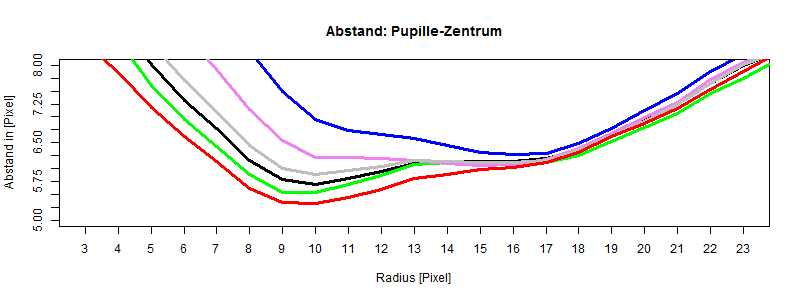
\includegraphics[width=\linewidth]{Eye_Img_Box/Vergleich_A}
	\caption{Median-Abstand in Pixel des Zentrums der Pupille gegen die Veränderung des Radius des Filters.\\
		Verfahren: Gleam (rot), Luminance (schwarz), Max (grün), Min (violett), New-Gleam (grau), Quadrat (blau)}
	\label{img_vergleich_A}
\end{figure}
\begin{figure}
	\centering
	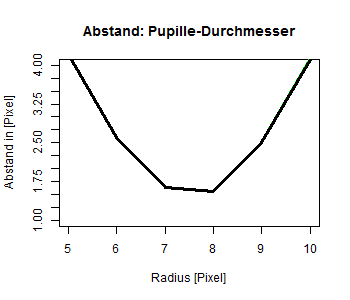
\includegraphics[width=0.49\linewidth]{Eye_Img_Box/Vergleich_P}
	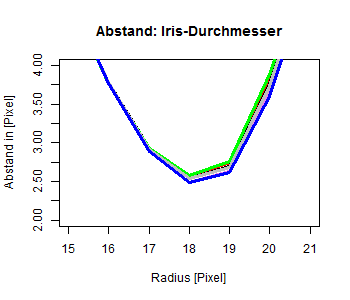
\includegraphics[width=0.49\linewidth]{Eye_Img_Box/Vergleich_I}
	\caption{Differenz zwischen den Radien gegen die Veränderung des Radius des Filters von Pupille (links) und Iris (rechts)\\
		Verfahren: Gleam (rot), Luminance (schwarz), Max (grün), Min (violett), New-Gleam (grau), Quadrat (blau)}
	\label{img_vergleich_PI}
\end{figure}
\subsection{Auswirkung der verschiedenen Graubild-Verfahren}
\label{grau_Auswirkung_ElSe}
Es zeigt sich, dass die Verfahren mit denen der Farbwert in einen Grauwert überführt wird, durchaus Auswirkungen auf die Qualität der Berechnung haben.\\
Für die Bewertung der Verfahren werden folgende Kriterien verwendet: Die Differenz zwischen den berechneten und tatsächlichen Radien von Pupille und Iris sowie die Abweichung des berechneten Zentrums der Pupille.\\
Der minimale Abstand der berechneten Zentren ergibt sich bei dem Gleam-Verfahren mit $5.327$ Pixel als Median, siehe \autoref{img_vergleich_A}. Der beste Radius für den Filter ist für die Position der Iris bei 10 Pixel.\\
Ein Unterschied zwischen den Verfahren konnte bei der Bestimmung des Radius der Pupille nicht gefunden werden, siehe \autoref{img_vergleich_PI} links. Der beste Radius für den Filter ist im Test bei 8 Pixel und ergibt eine Abweichung von $1,555$ Pixel.\\
Für die Bestimmung der Iris hat das quadratische Verfahren die geringste mittlere Abweichung mit $2,488$ Pixel, nur etwas genauer als Min-Verfahren ($2,49$ Pixel). Für diese Berechnung ist ein Radius des Filters von 18 Pixel am besten gewählt.\\
Somit wurden drei Verfahren ausgewählt um diese näher zu untersuchen, Gleam mit der geringsten Abweichung des Zentrums, Quadrat als bestes Resultat bei der Iris und Luminance da es ein Standartverfahren ist. Mit allen Verfahren wurde die Berechnung zur Pupille/Zentrum/Iris für verschieden groß skalierte Bilder bestimmt mit ihren jeweiligen optimalen Filterradien.\\
Bei der Berechnung der Pupille auf den unterschiedlich großen Abbildungen ist weiterhin kein Unterschied zu erkennen, siehe \autoref{img_Vergleich_Scal_PI} oben.\\
Auch bleiben die Unterschiede der Verfahren erhalten und die Fehler auf dem glichen Niveau bis zu einer Skalierung von $0,15$, ab welcher die Berechnung bei allen Verfahren scheitert. So liefert das Gleam-Verfahren die besten Ergebnisse im Bezug auf das Zentrum, wo hingegen das Quatrat-Verfahren geeignet für die Bestimmung des Iris-Radius ist.
\begin{figure}
	\centering
	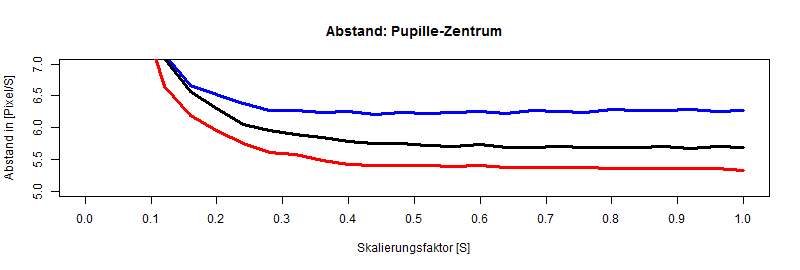
\includegraphics[width=\linewidth]{Eye_Img_Box/Vergleich_Scal_A}
	\caption{Euklidischer Abstand in Pixel zwischen dem berechneten Zentrum der Pupille und dem des Datensatzes gegen die Veränderung des Radius des Filters.\\
		Verfahren: Gleam (rot), Luminance (schwarz),  Quadrat (blau)}
	\label{img_Vergleich_Scal_A}
\end{figure}
\begin{figure}
	\centering
	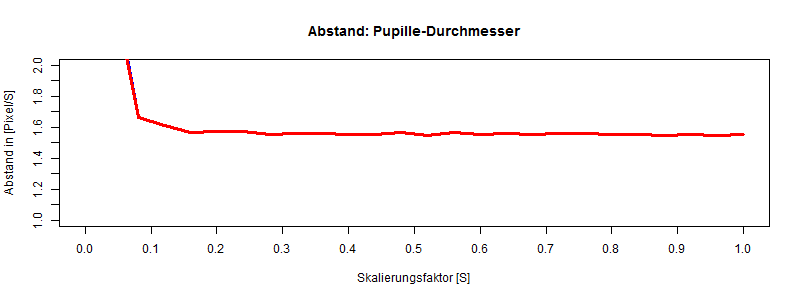
\includegraphics[width=\linewidth]{Eye_Img_Box/Vergleich_Scal_P}
	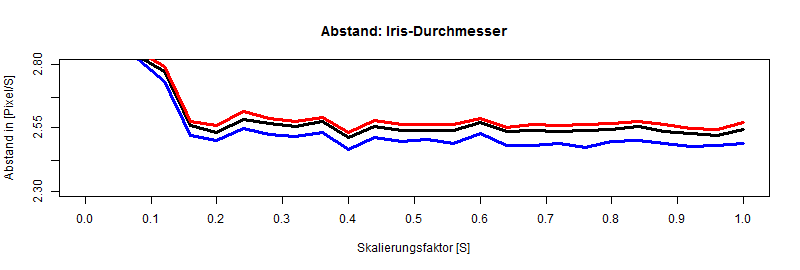
\includegraphics[width=\linewidth]{Eye_Img_Box/Vergleich_Scal_I}
	\caption{Differenz in Pixel zwischen den Radien der Berechnung und dem des Datensatzes gegen die Veränderung des Radius des Filters.\\ Oben: Pupille mit Filterradius 8, Unten: Iris mit Filterradius 18\\
		Verfahren: Gleam (rot), Luminance (schwarz), Quadrat (blau)}
	\label{img_Vergleich_Scal_PI}
\end{figure}
\subsection{Vergleich zu OpenFace}
Als Referenz wird das Ergebnis von OpenFace, für die zusätzlich bestimmten Landmarks der Augen, verwendet. Dies wurde auch auf dem Augendatensatz \cite{database_Eye} angewendet, um vergleichbare Ergebnisse zu erhalten.\\
Wird \autoref{OpenFace_Eye} mit \autoref{img_Vergleich_Scal_A} bzw. \autoref{ElSe_scall} verglichen so ist zu erkennen, das OpenFace im Mittel einen geringen Fehler bis zu einer Skalierung von $0,47$ besitzt als ElSe. Ab diesem Wert hat ElSe einen geringen mittleren Fehler, da die Abweichung fast unverändert bis $0,12$ beibehalten wird.\\
Da diese Qualität von ElSe nur erreicht werden kann, wenn es auf einem passenden Bildausschnitt angewendet wird, ist auch die Detektion des Auges von Interesse.\\
Aus \autoref{OpenFace_Eye_Box} ist zu entnehmen, dass der Bereich des Auges zwar nicht so exakt bestimmt wird, allerdings überdeckt er den relevanten Bereich ausreichend genau damit die Landmarks im Bildausschnitt liegen. Somit kann dieser Bildausschnitt als Eingabe von ElSe verwendet werden.
\begin{figure}
	\centering
	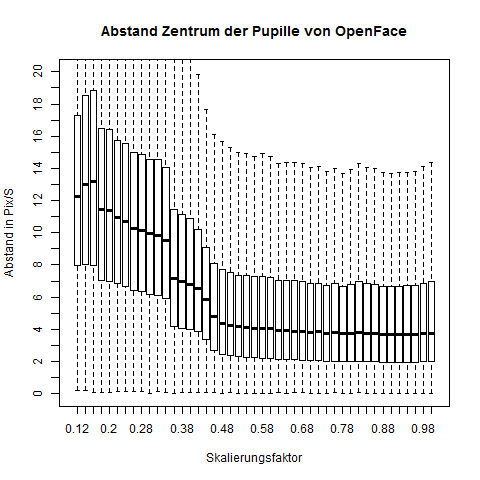
\includegraphics[width=0.49\linewidth]{Eye_Img_Box/Openface_PC}
	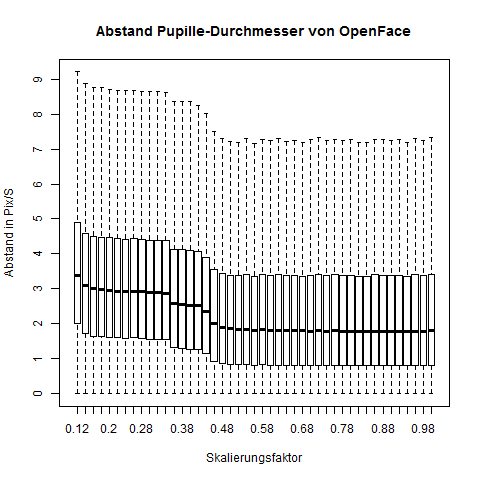
\includegraphics[width=0.49\linewidth]{Eye_Img_Box/Openface_PW}
	%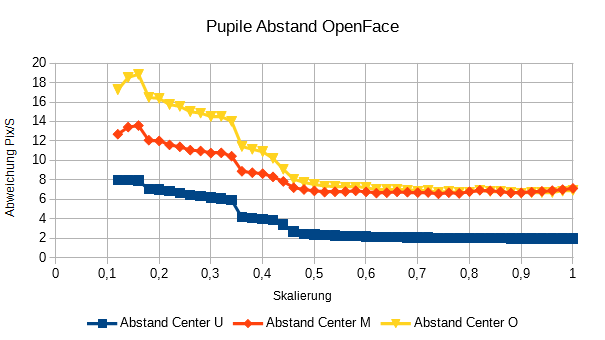
\includegraphics[width=0.45\linewidth]{Eye_Img/OpenFace_Zentrum_P}
	%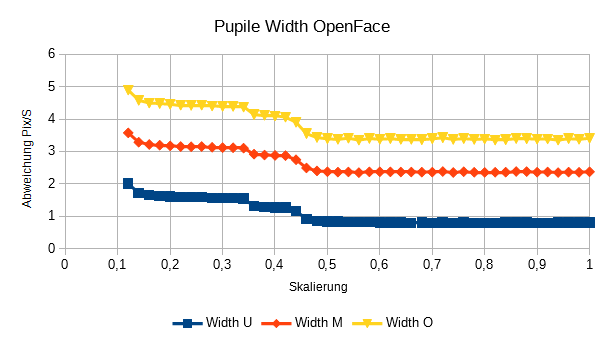
\includegraphics[width=0.45\linewidth]{Eye_Img/OpenFace_Width_P}
	\caption{Auswirkung der Bildgröße auf die Qualität der Augendetektion von OpenFace. Aufgetragen ist die Abweichung [Pixel/Skalierung] gegen den Skalierungsfaktor.}
	\label{OpenFace_Eye}
\end{figure}
\subsection{Ergebnis}
Die Tests haben ergeben, das ElSe mit einem Radius von 10 Pixel auf Bildern die mithilfe von Gleam ins Graue überführt wurde die besten Ergebnisse liefert. Dabei ist das Verfahren stabil gegenüber der Skalierung und kann die Iris bis zu einer Größe von 3 Pixel erkennen, das einer Distanz von etwa $4m$ entspricht (Basierend auf der Actioncam).\\
Allerdings hat der Vergleich ergeben, das bis zu einer Skalierung von $0,47$ ElSe schlechtere Ergebnisse liefert als das OpenFace-Augen-CNN.\\
So kann das Ergebnis von OpenFace bei Bilder in denen die Iris größer als 21 Pixel ist direkt als Lösung verwendet werden, da der mögliche Fehler von OpenFace geringer ist als der von ElSe.\\
Im Bereich zwischen 17 und 15 Pixel ($0,5-0,44$) können beide Ergebnisse kombiniert werden, da sie ungefähr gleich gute Ergebnisse liefern um den Gesamtfehler zu minimiren, da die beiden Verfahren unabhängig voneinander arbeiten.\\
Sollte die Iris im Originalbild noch kleiner sein, so ist ElSe deutlich genauer, da es noch bis zu einer Irisgröße von 3 Pixel stabil funktioniert.\\
Eine genauere Darstellung der Messergebnisse ist in \autoref{Abbildungen} dargestellt. Die Auswirkung der Radien und der verschieden Verfahren auf die Pupille ist in \autoref{ElSe_Gray_Pupille}, auf die Iris in \autoref{ElSe_Gray_Iris} und auf die Bestimmung des Zentrums in \autoref{ElSe_Gray_Zentrum} dargestellt, die Auswirkung der Skalierung in \autoref{ElSe_scall}.\\
Bei realen Aufnahmen sind Bildfehler unvermeidlich, so können Reflektionen (Brille, Kontaktlinse usw.), Make-Up und körperliche Eigenschaften wie Augenfarbe die Detektion erschweren. Ein Problem das schon im originalen Test \cite{ElSe} aufgetreten ist, wenn der Farbunterschied zwischen Iris und Pupille recht gering ausfällt oder durch Reflektionen der Kantenverlauf gestört wird, wodurch die maximale Distanz in der eine Auswertung der augen möglich ist weiter sinkt.